%2multibyte Version: 5.50.0.2953 CodePage: 1251

\documentclass{article}
\usepackage{hyperref}
\usepackage{url}
\usepackage{graphicx}

\begin{document}
	
	\title{How to Update the Equity Risk Premium Model
		\author{Eric Huang and (more recently) Charlie Smith}
		\date{\today}
	}
	
	\maketitle
	
	\section{ERP Background}
	
	The equity risk premium (ERP) is an important aspect in asset pricing. It is the difference between the expected returns on equities and the risk free rate. We estimate the ERP by combining data from twenty models that have been proposed in the literature. Check out \path{2015_EPR_equity-risk-premium.pdf} for an overview of this project. 
	
	\section{Repository Location}
	
	The bare repository for the Equity Risk Premium (ERP) Model is
	located in \path{\\ranhpc01-smb.ny.frbres.org\data\cmwbb\GitBareERP\ERP_Article.git}. Clone the repository to your RAN directory (rce) and make all changes there. When naming the local Git repository cloned from the remote \path{EPR_article.git}, please follow the proper program naming routine (no spaces, no rare characters, etc.) so that the
	program does not crash due to invalid directory.
	
	\section{Running ERP}
	\subsection{Tools Required}
	\begin{enumerate}
		\item Anaconda for Python 2.7, available \href{https://www.continuum.io/downloads}{here}.
		\item Matlab 2019b, with the Statistics and Machine Learning Toolbox.
		\item Stata version 16 or greater. 
		\item WRDS account, available \href{https://wrds-web.wharton.upenn.edu/wrds/}{here}.
		\item For FredFetch, you may need an api key, which is stored in the readme folder under api.txt. The FredFetch toolbox is saved in the \path{code/Matlab subfunctions} folder. To get a new FRED api key, create an account with \href{https://fred.stlouisfed.org/}{FRED} and then get an API key \href{https://research.stlouisfed.org/docs/api/api_key.html}{here}.
		\item This project is run on the RAN cluster with 25 GB of memory. 
	\end{enumerate}
	
	\subsection{Before Updating}
	
	\begin{enumerate}
		\item Change the variable ``root\_dir'' in the \path{run_all.m} to the location of the directory where your files (ERP Project) are stored. 
		\item After creating a WRDS account, go to the WRDS web portal \href{https://wrds-cloud.wharton.upenn.edu/SASStudio/}{here}, you will be prompted to enter credentials for SAS, enter your user name and password for your WRDS account. Now create a folder structure that matches the following image: 	
		\item 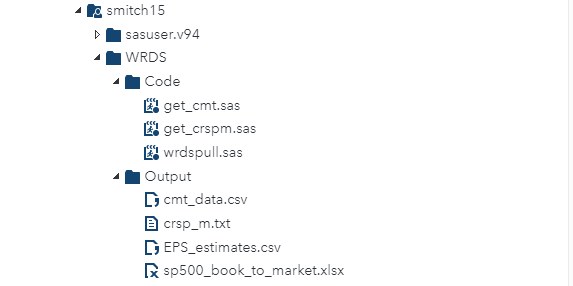
\includegraphics{WRDSfilestructure.PNG}
		\begin{enumerate}
			\item Inside your folder in WRDS, you need to create a folder called ``WRDS'' and within that folder two folders, one called ``Code'' and one called ``Output.'' 
			\item After doing so, go to \path{Code\project_scripts\download_data.m} and update the variables ``wrds\_code\_dir'' and ``wrds\_out\_dir'' to match the location of those two folders. In addition, change ``wrds\_username'' and ``wrds\_password'' to match your username and password. 
			\item When you eventually run \path{Code\project_scripts\download_data.m} , it puts the .sas files from \path{Code\wrds_scripts} into the code folder, runs the sas files in your WRDS folder, and then downloads the data.
		\end{enumerate}  
		\item Update the files that require manual updating, specifically \path{input\cfo_data.csv} and \path{input\tb1m.csv}. 
		\begin{enumerate}
			\item tb1m.csv - is a HAVER download that is transferred from the SAN to the RAN. The code to download this data is located in \path{code\san_ scripts\haver_data.do}. Run this do file in Stata locally on the SAN. Then load up WINSCP on your computer, navigate to the folder where the data was downloaded on the SAN and copy that data to \path{\Input} in ERP.
			\item cfo\_data.csv - requires manually updating the data using the CFO survey website, located \href{ https://cfosurvey.fuqua.duke.edu/release/}{here}. Go to the current year and quarter and select US high level results. Then find the part in the pdf where they report the expected average annual S\&P500 return over the next 1 and 10 years. The precise questions are: ``Over the next 10 years, I expect the average annual S\&P
			500 return will be:Expected return'' and  ``Over the next year, I expect the average annual S\&P 500	return will be:Expected return.'' Add the mean surveyed return and the number of total surveyed to the \path{\Input\cfo_data.csv} file for those two questions. 
		\end{enumerate}
	\item In \path{Code\project_scripts\cay.m} the url in line 35 should be updated. To do so, go to the Bureau of Economic Analysis website \href{https://apps.bea.gov/histdata/histChildLevels.cfm?HMI=7}{here}. Select the most recent version of data (e.g. 2020, Q1) and then under the main tab right click on section two. Select ``copy link address'' and then paste that in place of the url in line 35. 
	\end{enumerate}
	
	\subsection{Running ERP}
	
	\begin{enumerate}
		\item Open run\_all.m in the root folder of the ERP repository and run the file.
		\item Check to make sure the output seems reasonable (compare to previous vintages).
		\item If everything works, make a commit. 
	\end{enumerate}
	
	\subsection{Areas where things break}
	\begin{enumerate}
		\item Shiller data has broken (code stops running) due to changes in the websites data format. If this occurs, the code will break in NY\_Fed\_CM\_DAPM.m. 
		\item The WRDS download can sometimes break when downloading crsp\_m.txt. I put it in a try catch command to keep the code running. If it is not downloading, you can download it manually To do so:
		\begin{enumerate}
			\item Log into WRDS SAS Studio. 
			\item Find the file in your folder structure.
			\item Right click on the file and download it.
			\item Transfer it to the \path{\Input}.
		\end{enumerate}
	\end{enumerate}
	
	\section{Project/Folder Outline}
	
	\subsection{run\_all.m}
	
	This file runs the entire ERP project. Ideally, we will reach the situation where all that needs to happen is click run on this file. It takes around 20 minutes to run in Matlab2019b interactive session, with \path{Code\project_scripts\download_data.m} occupying around 15 minutes. 
	
	\subsection{Code}
	
	This folder contains all the code to run the project. The code is sorted into a variety of folders. The scripts that are called by \path{run_all.m} are stored in \path{code\project_scripts}. Functions are stored in three separate folders, specifically \path{code\functions}, \path{code\Matlab subfunctions}, and \path{code\NYFed_functions}. There are a few python (stata) scripts that are called by the .m files in \path{code\project_scripts}, that are stored in \path{code\python_scripts} (\path{code\stata_scripts}). Finally, the scripts that are run in WRDS are stored in \path{code\wrds_scripts}. run\_all.m calls files from \path{code\project_scripts}, which use functions from the various function folders and calls stata, python, and wrds.sas files occasionally. 
	
	\subsection{Input}
	
	This folder contains all the raw data that is needed to run the ERP project. 
	
	\subsection{Temp}
	
	This folder contains data at various stages of the project. Each folder maps to a script in the \path{code\project_scripts} folder. Each folder contains an input folder and an output folder. The input is the data that enters that script and the output is the data produced by the script. 
	
	\subsection{Output}
	
	This folder contains all the output. The most important files are: 
	
	\begin{enumerate}
		\item \path{Original_data.csv} contains information on the input data, its sources, and the dates it spans. Use this to identify which datasets are updating and which are not. 
		\item \path{Constructed_variables.csv} contains information on the variables that this project constructs. Similarly, use this to identify which variables are updating and which are not. 
		\item \path{ERP_1yr_ahead.csv} contains time series on the 20 models this project computes and uses. Similarly, use this to identify which models are updating and which are not. 
		\item \path{ERP_principal_components.csv} contains the ERP estimates at different time horizons. This is the main output. 
	\end{enumerate}
	
	\subsection{BW}
	
	This folder, located in the code folder, includes data and files necessary to replicate the Baker Wurgler investor sentiment measure. I have almost replicated the measure, we are just missing two data-series necessary to construct it, specifically the dividend premium and the closed end fund discount. The code is written in such a way that once are those completed, it just has to be included in to the collect\_data.m script where bw data is currently accessed. 
	
	In addition, two of the data-series for this measure necessitate downloading them on the san. They are the issuance of equity and debt. To do so, run \path{code\san_scripts\issuance_download.m} on the SAN and then transfer the two csvs to the RAN input folder.
	
	You can check their website \href{http://people.stern.nyu.edu/jwurgler/}{here} to see if they have updated their data. The most recent version runs until December 2018. 
	
	\section{State of Project February 2020}
	
	All data in \path{Output\original_data} is updated until late 2019, except for sentiment, equity issuance, and debt issuance. Those variables are all part of Baker Wurgler.  
	
	In \path{Output\Constructed_variables} the same holds true. Here all variables are updated until at least September 2019, except the Baker Wurgler variables listed above. 
	
	In \path{Output\ERP_1yr_ahead} all models are updated until September 2019 except, Model 8, Model 9 and 10 (which are annual), Model 18, Model 19 (which is the Baker Wurgler model), and model 20 (which is quarterly). These exceptions have all been updated between December 2018 and July 2019. 
	
	\section{Next Steps}
	\begin{enumerate}
		\item Replicate BW and include automatically updating BW in the project.
		\item Automate tb1m.csv
		\item Automate cfo\_data.csv but most likely is not worth it. 
	\end{enumerate}
	
\end{document}
